
\section{Statement of Work (SOW)}
The project's aim is to develop a minaturized high-sensitivity, low-noise magnetic gradiometer. Our approach is to mimic the mechanism found in magnetosomes, the specialized cells four from bacteria to higher vertebrates such as fish and birds (see \ref{sec:inno}). This is comprised of four main tasks: modeling and simulation, microfabrication process design, circuit design, and device manufacture and testing. Each Phase (I,II,III) will include these four tasks.

\subsection{Phase I}

AMBIIENT Phase 1 will demonstrate sensor functionality and performance in a laboratory
setting meeting the performance metrics as indicated in Table \ref{table:obj}. 

\subsubsection{Modeling and simulation}\label{sec:p1:em}
\begin{itemize}
\item The objective in this phase is to simulate the MEMS device, taking into account geometry, material properties, and multiphysics interactions, in order to determine the range of acceptable design options. In addition, scaling laws will be derived, such that a scale model of the sensor could be fabricated from COTS components.
\item Our approach here is to initially specify geometry and physical properties by hand calculation, the investigae more deeply in a finite-element multiphysics solver.
\item This task will be accomplished at UF by Joaquin Casanova.
\item Completion of this task is specified by successful simulation of the MEMS device that meets the physical requirements specified in the BAA.
\item Deliverables include successful simulation results and design parameters.
\item No government equipment is required.
\item To reduce risk of later failure due to non-manufacturability, this task will be accomplished within fabrication constraints specified by the MEMS team at UF. This ensures the design is physically realizable. In parallel, other sensing modalities could be explored in the case that the MEMS cantilever is not practical.
\item This task will be accomplished at UF.
\end{itemize}
\subsubsection{Microfabrication}
\begin{itemize}
\item The objective in this phase is to develop a microfabrication strategy (materials, deposition, patterning) that can meet the requirements found from simulation.
\item Our approach here is to find a range of dimensional constraints and material types that could be physically realizable.
\item This task will be accomplished at UF by Dr. YK Yoon.
\item Completion of this task is specified by successful specification of a microfabrication plan for the sensor described by the simulation results.
\item Deliverables include successful microfabrication plan.
\item No government equipment is required.
\item To reduce risk of later failure due to non-manufacturability, this task will be accomplished with paralel investigating of alternative MEMS sensing modalities.
\item This task will be accomplished at UF.
\end{itemize}
\subsubsection{Circuit design}
\begin{itemize}
\item The objective in this phase is to develop a circuit which amplifies and digitizes the the voltage produced by the MEMS elements.
\item Our approach here is to ...
\item This task will be accomplished at TTU by Dr. Changzi Li.
\item Completion of this task is specified by successful design of a circuit capable of amplifying and digitizing MEMS output voltage with input-referred voltage noise low enough to meet the overall sensitivity requirement.
\item Deliverables include successful design and prototype of the circuit, usable with the scale model, using COTS components.
\item No government equipment is required.
\item To reduce risk of later failure due to excessive noise, this task will investigate only specifically low-noise designs.
\item This task will be accomplished at TTU.
\end{itemize}
\subsubsection{Manufacture and testing}
\begin{itemize}
\item The objective in this phase is to construct a scale model of the MEMS design using COTS components, according to the scaling law developed in \ref{sec:p1:em}.
\item Our approach here is to mimic the MEMS structure with COTS materials (ie, commercially available piezo elements and magnetic sheets)
\item This task will be accomplished at UF by Dr. Joaquin Casanova.
\item Completion of this task is specified by successful construction and testing of a scale model, which satisfies Table \ref{table:obj} after application of scaling laws.
\item Deliverables include successful scale model prototype of the sensor.
\item No government equipment is required.
\item To reduce risk of failure, prototyping will begin early in Phase 1.
\item This task will be accomplished at UF.
\end{itemize}
\subsection{Phase II}
  
AMBIIENT Phase 2 will develop and demonstrate an integrated sensor head meeting the
performance and SWaP metrics of Table \ref{table:obj}, and including all vacuum, photonic, and thermal
control components.

\subsubsection{Modeling and simulation}
\subsubsection{Microfabrication}
\subsubsection{Circuit design}
\subsubsection{Manufacture and testing}
\subsection{Phase III}
AMBIIENT Phase 3 will demonstrate a fully integrated gradiometer comprising all control
electronics, power conditioning, and packaging, meeting all performance metrics of Table  \ref{table:obj}

\subsubsection{Modeling and simulation}
\subsubsection{Microfabrication}
\subsubsection{Circuit design}
\subsubsection{Manufacture and testing}

\section{Innovative Claims}\label{sec:inno}

Our approach is to design a sensor based on a magnetoreceptive mechanism used in nature - magnetite crystals torqued by external magnetic fields open ion channels in the cell wall. To mimic this, we propose a microfabricated MEMS sensor, with a layer of magnetic material on top of piezo electric cantilevers. When forced with an exernal field, torque induced on the magnet create stress in the piezo, and thus a voltage is produced. There are three advantages to this approach. First, microfabrication allows for a small size. Second, by orienting individual sensing elements in anti-series order, the output is natively a gradiometer. Third, by selecting the resonant frequency of the cantilever carefully, we can create a gradiometer which outputs a spectrogram directly. Though fluxgates can be microfabricated and function as gradiometers, they suffer a size/sensitivity tradeoff. Microfabricated atmonic magnetometers are sensitive but don't function natively as gradiometers. Other micro-scale magnetometers, namely Lorentz-type, which operate on a similar mechanism, are not yet sensitive enough and haven't been used as frequency-domain gradiometers, as in the proposed design.

\section{Detailed Technical Approach}

Magnetometers serve an important role in investigating biologically generated electromagnetic fields, such as those created by neuronal currents, or geological magnetic fields. Typically, magnetometers are unable to achieve high sensitivity in an ambient, unshielded environment - getting to femtotesla level sensitivity requires magnetic shield and cryogenic sensors, such as SQUID \cite{lenz2006magnetic}. The novel spin relaxation free magnetometer has been minaturized and achieves less than 10 fT/$\sqrt{Hz}$, but still requires shielding and lacks directional sensitivity \cite{shah2013compact}. Fluxgates have achieved pT level resolution at small size, but this is insufficient for biomagnetic field measurement \cite{sasada2002orthogonal,uchiyama2014highly,sasada2014fundamental} 

\begin{figure}[h]
  \centering
  \begin{subfigure}
    \centering
    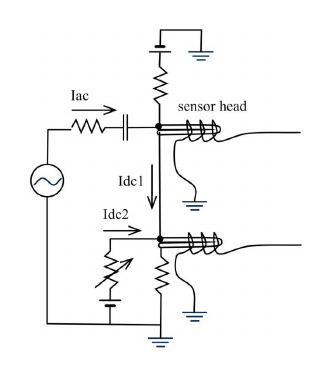
\includegraphics[width=0.5\textwidth]{fmofg}
  \end{subfigure}
  \begin{subfigure}
    \centering
    
\includegraphics[width=0.5\textwidth]{fmofg2}
  \end{subfigure}
\caption{Fundamental-mode orthogonal fluxgate gradiometer \cite{sasada2014fundamental}.}
\label{fig:fmofg}
\end{figure}
Lorenz-type magnetometers (which translate magnetic fields into mechanical actuation of a magnet or current carrying wire) have been built in MEMS substrates, but are as yet insufficiently sensitive and require shielding \cite{sinha201627,kyynarainen20083d,kumar2015ultra,thompson2009parametrically}

\begin{figure}[h]
\centering
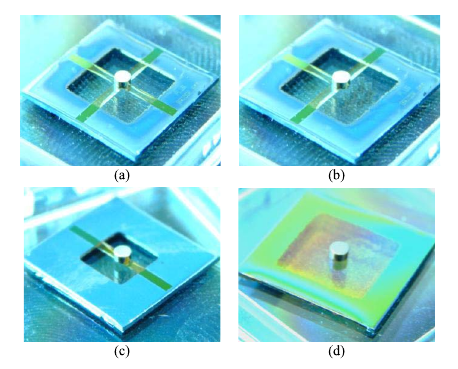
\includegraphics[width=0.5\textwidth]{lorenz}
\caption{Lorenz-type magnetometer \cite{sinha201627}.}
\label{fig:nd_lorenz}
\end{figure}

\begin{figure}[h]
\centering
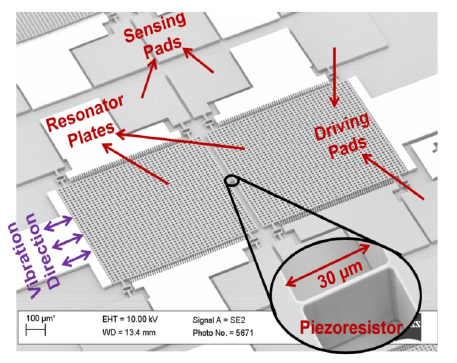
\includegraphics[width=0.5\textwidth]{lorenz2}
\caption{Lorenz-type magnetometer \cite{kumar2015ultra}.}
\label{fig:lorenz}
\end{figure}

In nature, many organisms have a sense of magnetoreception used for navigation, from magnetotactic bacteria to birds. Two mechanisms have been proposed: a spin-selective (and thus field-sensitive) chemical reaction rate, or magnetite crystals which are actuated by external fields and activate ion channels in the cell membrane \cite{johnsen2005physics,dodson2013radical,kirschvink2001magnetite}. Measurements of these magnetosomes show a magnetic dipole moment of up to 100fA/m$^2$ \cite{hanzlik2002pulsed,eder2012magnetic}.

\begin{figure}
\centering
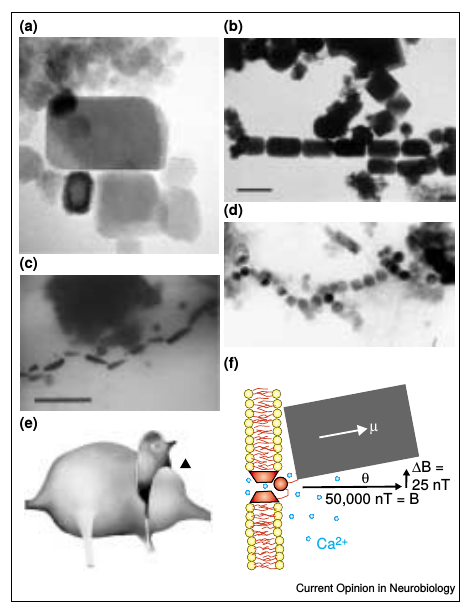
\includegraphics[width=0.5\textwidth]{kirsh2001}
\caption{Magnetosomal mechanism \cite{kirschvink2001magnetite}.}
\label{fig:magnetsosome}
\end{figure}

Our approach is to mimic the approach found in magnetosomes, with some key modifications so that is frequency-selective and functions inherently as a gradiometer and thus does not require shielding. The closest biomimetic sensor is a flow sensor which uses ferromagnetic cilia to detect microfluidic flow rates \cite{alfadhel2014magnetic}.

\begin{figure}[h]
\centering
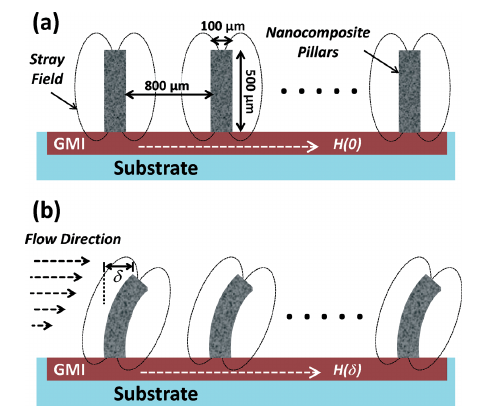
\includegraphics[width=0.5\textwidth]{cilia}
\caption{Magnetic cilia flow sensor \cite{alfadhel2014magnetic}.}
\label{fig:cilia}
\end{figure}

To acomplish this, we propose layering single-domain magnetic crystals on top of piezoelectric cantilevers. The moment $M$ induced on the magnetic layer with moment $\vec{\mu}$ and field $\vec{B}$ is:


$$  M=\vec{\mu} \times \vec{B} $$

Interpreted as a point load at the cantilever tip, this moment causes a stress distribution on a cantilever of length L, thickness t, second moment I, piezoelectric constant $g_{31}$, and modulus E, at point x, of

$$ \sigma=\frac{Mt(L-x)}{2I} $$

and $n$ in series generates a voltage

$$ V=\int_0^L\frac{Mt(L-x)}{2LI}g_{31}ndx $$

 Two features are possible from the cantilever design: frequency selection and gradiometery. As in \cite{shen2008design}, a cantilever has a resonant frequency, which can be modifying through geometrical parameters. Peak response will be achieved at this frequency. By selection many cantilevers of different dimensions, each corresponding to a separate output, the magnetometer output is a spectrometer. Many cantilevers at the same resonance in series generate a largeer voltage; in anti-series, the difference is taken, thus functioning as a gradiometer with very high spatial resolution. 

 Even though biological magnetoreception is limited to nT sensitivity, our design will allow us to surpass this. First, by careful selection of materials (such as Co-Pt or rare-earth magnets) \cite{coey2010magnetism, arnold2009permanent} we can have much higher magnetic dipole moment, and thus higher moment. Second, by careful selection of geometery, we can employ parametric resonance \cite{van2006resonant}. Finally, using two banks of cantilevers in series in anti-series, we both boost the voltage and create a high resolution gradiometer.

 The noise floor of magnetic materials is governed by Barkhausen noise - the random flipping of magnetic domains \cite{butta2012sources}; this noise is characterized as a flux noise level. The flux noise can be converted into a magnetic moment noise, and thus moment noise. Piezo noise floor is largely a function of piezo losses \cite{levinzon2004fundamental}. Additionally, there is the input-referred noise of any amplifier. With conservative estimates for all of these, and two anti-series banks of 30 cantilevers each with dimensions 400x40x3 $\mu$m, the sensitivity level is less than 10 fT/cm/$sqrt{Hz}$.

 An alternative design, should magnetic/piezo integration prove infeasible, is to measure the tilt of magnetic cilia  by some other means. One way would be to affix micromirrors to the magnetic cilia and measure the change in reflected angle of a laser beam \cite{duan2016optical}. Instead of a laser, millimeter-wave radar could detect changes in tilt angle, similar to the techniques used in vital-signs radar \cite{li2013review}.
 
\begin{figure}
\centering
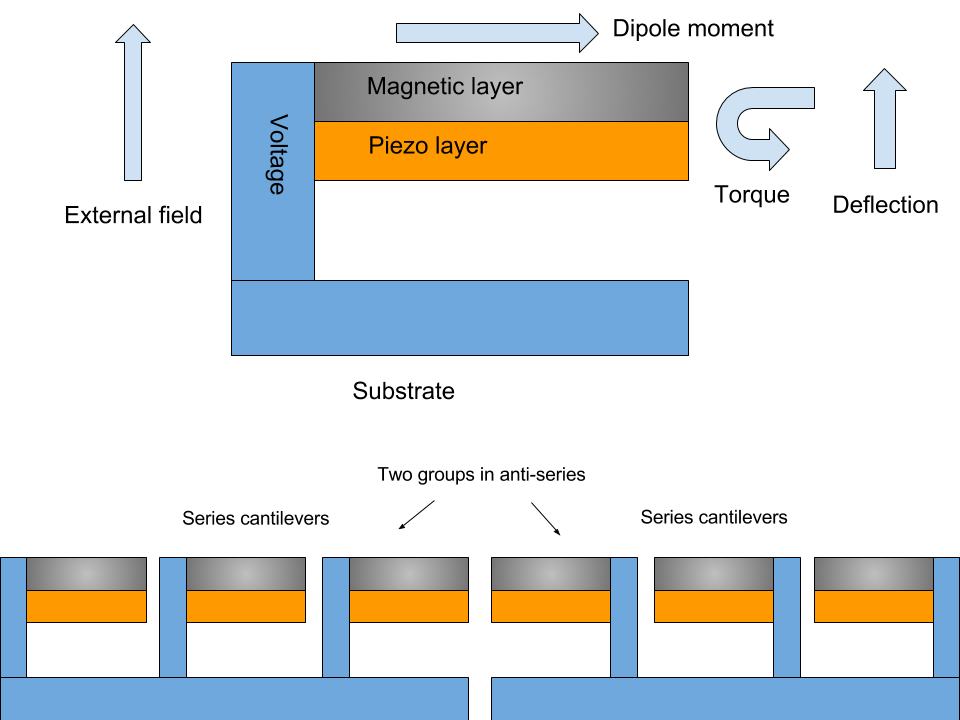
\includegraphics[width=0.75\textwidth]{biomag}
\caption{Diagram of proposed design.}
\label{fig:diagram}
\end{figure}

MEMS fabrication processes are capable of constructing the above-described sensor. This consists of two main fabrication tasks: piezo cantilever construction, and magnetic material integration. The process described in \cite{shen2008design} can be used for our task, with an additional step to apply the magnetic layer. PZT has a high voltage coefficient and is highly suitable for the piezo elements \cite{tadigadapa2009piezoelectric} and can be deposited with pulsed laser deposition or solution-based deposition and patterned with chemical etching or ion etching. Rare-earth magnetic materials, such as alloys of Sm-Co, offer high magnetic energy product at room temperature and can be integrated into MEMS using sputtering or pulsed laser deposition \cite{arnold2009permanent}. However, patterning of these materials is slow, using wet etching or ion-beam milling.  

Circuit description?

To test, in Phase I, it may be more feasible to test a scale model which can be built from COTS components. An appropriate scaling law and set of nondimensional parameters can be used to appropriately choose materials and dimensions for the scale model.

\begin{table}[h!]
\centering
  \begin{tabular}{|c||c|c|c|}
    \hline
    Metric & Phase 1 & Phase 2 & Phase 3 \\
    \hline
    \hline
    Power consumption & 150 mW & 50 mW & 100 mW \\
    \hline
    Sensor Volume & 3x3x10 cm & 1x1x7 cm & 1x1x7 cm \\
    \hline
    Control Electronics Volume  & N/A & N/A & < 20cm$^2$ \\
    \hline
    Ambient Magnetic Field & $\pm$ 100 $\mu$T & $\pm$ 100 $\mu$T & $\pm$ 100 $\mu$T \\
    \hline
    Ambient Operating Temperature & N/A & 0$^{\circ}$ C to 50$^{\circ}$ C & 0$^{\circ}$ C to 50$^{\circ}$ C \\
    \hline
    Gradient Full-scale Range & 1 nT/cm & 1 nT/cm & 1 nT/cm \\
    \hline
    Gradient Sensitivity & 10 fT/cm/$\sqrt{Hz}$ & 3 fT/cm/$\sqrt{Hz}$  & 1 fT/cm/$\sqrt{Hz}$ \\
    \hline
    Gradient Accuracy & 100 fT/cm & 30 fT/cm & 10 fT/cm \\
    \hline
    Total Field Range & 100 $\mu$T & 100 $\mu$T & 100 $\mu$T \\
    \hline
    Total Field Sensitivity & 100 pT/$\sqrt{Hz}$ & 30 pT/$\sqrt{Hz}$  &  10 pT/$\sqrt{Hz}$ \\
    \hline
    Total Field Accuracy & 1 nT & 500 pT & 100 pT \\
    \hline
    Data Rate & 100/s & 200/s & 500/s \\
    \hline
    3 dB Bandwidth & 200 Hz & 400 Hz & 1000 Hz\\
    \hline
  \end{tabular}
\caption{Design objectives, by phase.}
\label{table:obj}
\end{table}

\begin{table}[h!]
\centering
  \begin{tabular}{|c||c|c|}
    \hline
    Phase & Milestone & Date\\
    \hline
    \hline
    1 & Cantilever simulation and design & \\
    \hline
    1 & Fabrication plan & \\
    \hline
    1 & Circuit design & \\
    \hline
    1 & Scale model design and testing & \\
    \hline
    \hline
    2 & Cantilever simulation and design & \\
    \hline
    2 & Fabrication plan & \\
    \hline
    2 & Circuit design & \\
    \hline
    2 & MEMS fabrication and testing & \\
    \hline
    \hline
    3 & Cantilever simulation and design & \\
    \hline
    3 & Fabrication plan & \\
    \hline
    3 & Circuit design & \\
    \hline
    3 & MEMS fabrication and testing & \\
    \hline
  \end{tabular}
\caption{Milestones schedule}
\label{table:sched}
\end{table}

\section{Risk Analysis and Mitigation Plan}

\begin{table}[h!]
\centering
\begin{tabularx}{.85\textwidth}{|X||c|c|X|}
    \hline
    Risk & Probability & Impact & Plan\\
    \hline
    \hline
    Insufficient sensitivity in simulation & 3 & 10 & Change to alternate design \\
    \hline
    Best available MEMS processes infeasible & 4 & 10 & Change to alternate design \\
    \hline
    Scale model inaccurate method for initial testing & 3 & 5 & Rely on MEMS fabricated sensor for test \\
    \hline
    Fabrication time/window exceeds deadlines & 3 & 5 & Extend project time \\
    \hline
    Circuit/sensor fails tests & 3 & 9 & Identify points of failure for next design \\
    \hline
\end{tabularx}
\caption{Risk matrix}
\label{table:risk}
\end{table}

Identify the major technical and programmatic risks in the program. Include a risk matrix.
For each risk, assign a probability of occurrence on a scale of 1-10, where 10 indicates a high
likelihood that the risk will impact program success, as well as an assessment of impact, also
on a scale of 1-10, where 10 indicates that this risk would maximally limit the program from
delivering prototypes on schedule or meeting performance objectives. For each item with
total risk (likelihood × impact) exceeding 40, include a plan for mitigating the risk and
assessing risk reduction.
Where necessary, parallel risk reduction tasks may be proposed, e.g. concurrent development
of redundant techniques or components. The proposal must differentiate the primary
technical path from risk reduction tasks, which should be uniquely identified in the SOW and
separately costed as optional tasks in Volume II.

\section{Schedule and Milestones}
Include a high-level Gantt chart outlining major technical tasks and measureable milestones
by phase. At a minimum, the schedule should include each SOW task of Volume 1, Section
II.A. Where risk reduction tasks are proposed, the schedule should include a milestone for
assessment and removal of redundant tasks.

\section{Test Plan}
Describe how compliance with the proposed metrics and milestones will be demonstrated in
each phase of the program. The test plan should be structured so that compliant performance
can be verified prior to delivery of hardware for government test and evaluation.
\subsection{Phase 1}

\subsection{Phase 2}

\subsection{Phase 3}

\section{Results and Technology Transfer}
Description of the results, products, transferable technology, and expected technology
transfer. This should also address mitigation of life-cycle and sustainment risks associated
with transitioning intellectual property for U.S. military applications, if applicable. See also
Section IV.B.10, “Intellectual Property.”

\section{Ongoing Research}
Comparison with other ongoing research indicating advantages and disadvantages of the
proposed effort.
\section{Proposer Accomplishments}
Discussion of proposer’s previous accomplishments and work in closely related research
areas. In this section, also include any ongoing research projects or pending proposal activity
that technically overlaps with the proposed effort, including funding source, administrative
point of contact, and the program management plan for combining and de-conflicting the
efforts.
\section{Facilities}
Description of the facilities that will be used for the proposed effort.
\section{Teaming}
Description of the formal teaming agreements that are required to execute this program.
Describe the programmatic relationship between investigators and the rationale for choosing
this teaming strategy. Present a coherent organization chart and integrated management
strategy for the program team. For each person, indicate: (1) name, (2) affiliation, (3)
abbreviated listing of all technical area tasks they will work on with roles, responsibilities,
and percent time indicated, (4) discussion of the proposers’ previous accomplishments,
relevant expertise and/or unique capabilities.
